\section{Experiment Flow}
To start off the process, we wanted to create an overall architecture for the experimental process similar to the one shown in \textbf{\autoref{fig:DataArchitecture}}. The data is being prepared for each individual experiment in the \textit{Feature Engineering} phase before reaching the \textit{Experiments} phase.

\begin{figure}[H]
    \centering
    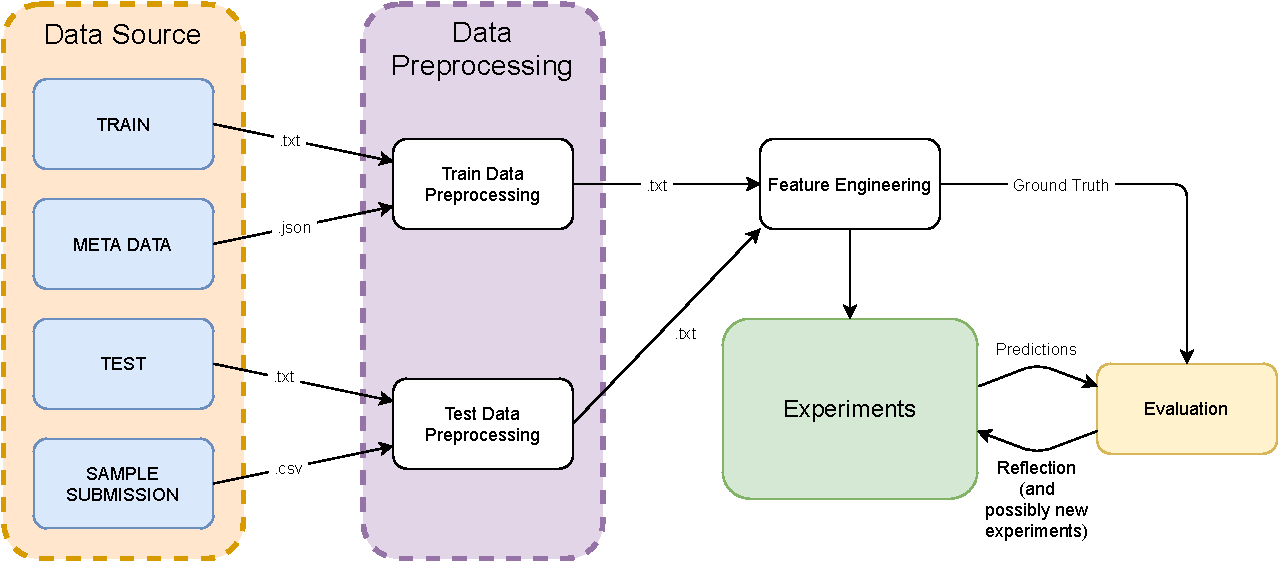
\includegraphics[scale=.7]{Images/Experiments/ExperimentFlow.pdf}
    \caption{The overall architecture with added evaluation.}
    \label{fig:experimentflow}
\end{figure}

As seen on \textbf{\autoref{fig:experimentflow}}, we have expanded on the \textit{Experiments} component to also interact with the \textit{Evaluation} component. This new component takes the ground truth data and compares it to estimations from the experiment. For this purpose, the \textit{Feature Engineering} component now passes the data to the \textit{Experiments} component and also the ground truth data to the \textit{Evaluation} component. The \textit{Evaluation} component now compares the result of the experiment to the ground truth and thereby evaluates the experiment. These results can be reflected on, which might lead to new experiments, which is indicated by the interaction from the \textit{Evaluation} component to the \textit{Experiment} component.

\subsection{Experiments}
The \textit{Experiments} component in \textbf{\autoref{fig:experimentflow}} represents the implementation and use of the positioning methods, mentioned in \textbf{\autoref{sec:problemstatement}}, which we would need to test. The different experiments will include \gls{gbdt}, \gls{ann}, \gls{imu}-based methods and hybrids. Each experiment takes the input data from the \textit{Feature Engineering} phase. As mentioned in \textbf{\autoref{sec:datapipeline}}, this component is concerned with processing the data for the specific positioning method in the experiment. After receiving the data from the \textit{Feature Engineering} component, the implementation of the experiment will be executed to achieve estimations of the indoor locations. The estimations from these experiments will then be forwarded to the \textit{Evaluation} phase to determine the performance of the model.
%Elaborate the Experiment part of the design
%Generelt om hvad et eksperiment er + hvilke eksperimenter vi prøver af
%Kontekst til de andre dele (data pipeline + evaluation)
%Input og output til experiments
%

\subsection{K-Fold Cross Validation}
For the evaluation of our learning-based positioning methods, we will be using K-Fold Cross Validation. K-Fold Cross Validation is a statistical method used to evaluate machine learning models on a limited data sample and is ideal for selecting the optimal set of hyper-parameters to train a final model. K-Fold Cross Validation enables the option to use the entire dataset for training and testing the machine learning models compared to techniques like splitting the dataset into training, validation and test sets, and using these datasets to train and validate the model. It is also a useful way to test multiple machine learning methods to evaluate which of the methods works best for the data. 
The idea with K-Fold Cross Validation is to split the dataset into equally sized $K$ groups and use one of the groups as a validator to evaluate the performance of the models. This process is executed $K$ times where the group being the validator is shifted between the groups.\cite{kfold}

\begin{figure}[H]
    \centering
    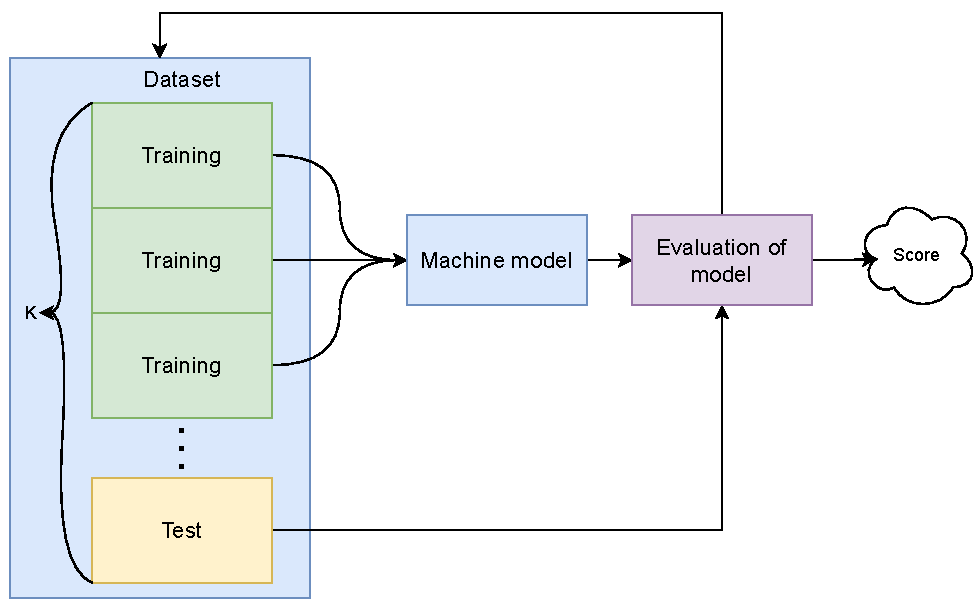
\includegraphics[scale = 0.7]{Images/Experiments/k_fold.pdf}
    \caption{Process on K-Fold Cross Validation.}
    \label{fig:kfold}
\end{figure}

As seen on \textbf{\autoref{fig:kfold}}, the dataset is split into $K$ groups, where $K-1$ groups will be used to train a machine learning model. The model will then be evaluated on the validator partition based on metrics. Afterwards, the validator will be shifted to another group and the machine learning model will be trained and get a score. This will be executed until all groups have been the validator. Each model will be discarded after the evaluation such that a new model is trained and evaluated in each iteration. The scores would then be summarized and will be the score for said model.
This procedure can be used on multiple models to compare the scores and determine the better model.

The value of $K$ can be configured, and a poorly chosen $K$ can result in poor performance. According to \cite{kfold_configk}, the choice of the value for $K$ is usually 10 since the value has shown an empirical test error rate which experienced best performance.    

\subsection{Evaluation}
To evaluate the different experiments, which is depicted as the \textit{Evaluation} component in \textbf{\autoref{fig:experimentflow}}, we have decided to implement a generic evaluator, which can be used to evaluate the different models/algorithms in terms of different performance metrics.
This evaluator should evaluate the result with regards to \textbf{\autoref{eq:rmse}} on X-, Y- and floor-coordinates, separately, where $v'$ denotes the ground truth coordinate value and $v$ denotes the estimated coordinate value. Additionally, the evaluator should also calculate the position error with regards to each estimation made by the algorithm or model. This evaluator will be used when comparing the different positioning methods. However, when considering the experimentation internally for the positioning methods, we will use the appropriate metrics for each positioning method instead of the metrics defined in the generic evaluator. For instance, it makes sense to consider the loss per epochs to identify possible performance bottlenecks for deep learning models.

\begin{equation}
    \text{\gls{rmse}} = \frac{1}{n} \sum_{i = 1}^{n} \sqrt{(v_{i}' - v_i)^2}
    \label{eq:rmse}
\end{equation}

The evaluator takes the position estimations from the \textit{Experiments} phase and the ground truth data from the \textit{Feature Engineering} component as input. From this, it is possible to calculate the \gls{rmse} of each position coordinate and the position error for each individual estimation. All of the performance metrics as well as the input to the evaluator should be recorded to a file dedicated for the evaluation output. The execution of the generic evaluation class should be integrated into each experiment, where it is possible to work with the results and maybe add additional evaluations.

%It should be noted that the \gls{pdr} algorithm will be evaluated differently since it is only able to estimate positions on a 2-dimensional level. \gls{pdr} will be still be evaluated by each of its position estimations, but will also use \textbf{\autoref{eq:MeanPositionError}} defined in \textbf{\autoref{sec:kaggleComp}} for its overall performance on each path.

% NOTER: 
% - Eksperimenter evalueres af single, central evaluator.
% Evaluate waypoints individually with position error
% Evaluator outputter resultater for hver enkelt waypoint.
%   Output indeholder ground truth, estimering, og position error for hvert enkelt prediction.
%   Output konkluderer med mean position error.
% Evaluatator tager ground truth data og estimeringer som input og udregner de nødvendige evalueringer og skriver dem i sidste ende til filer.
% Eksekvering af evaluator skal ske som en integreret del af hvert enkelt eksperiment.
% Evaluator skal generere output i 'results' folder.

\subsection{Frameworks and Libraries}
For implementing the different experiments and the generic evaluation class, we have decided to use the programming language Python for consistency with the development of the data handling. Furthermore, most of the methods or techniques, which we would like to implement and test, are supported in Python in terms of frameworks and libraries, making it the ideal programming language for this.

To implement these experiments, we will be using different frameworks and libraries. For some of the experiments, we have decided to use TensorFlow, which is an open-source machine learning platform, which contains implementations of the different machine learning algorithms that we want to experiment with.\cite{TensorFlow}

We also use the Light Gradient Boosting Machine (LightGBM) framework for some experiments. It is a machine learning framework and is designed to use tree-based learning for higher efficiency and better distribution of workload. This framework also contains an implementation of K-Fold Cross Validation.\cite{LightGBM}

LightGBM utilises the library sci-kit learn to perform the calculations for the models. Sci-kit learn consists of several different algorithms which are used by LightGBM. In this way, LightGBM acts as a structuring framework to help utilise the functionality of sci-kit learn.\cite{scikit}

As mentioned in \textbf{\autoref{sec:pdr}}, we will use the \gls{ahrs} toolkit for the heading estimation in the \gls{pdr} algorithm, which is a Python toolkit for attitude estimations. More specifically, we will use the Madgwick and the Extended Kalman Filter from \gls{ahrs}.\cite{ahrs}

% Vi bruger Python til det hele udover til wrapper til libs.
% TensorFlow (Neural network, HMM, knn og RNN)
% LightGBM

%\subsection{Coding Standard}
% - Kommentar på alle metoder/funktioner/procedurer.
%   - Kommentarer skal komme den sidste linje før deklaration.
% - Snake-case til symbol deklarationer.
% - 